\documentclass[conference]{IEEEtran}
\usepackage[T1]{fontenc}
\usepackage{graphicx,booktabs,amsmath,array,url}
\usepackage[hidelinks]{hyperref}
\usepackage{tikz}
\usetikzlibrary{arrows.meta,positioning}
\usepackage{balance}
\newcommand{\code}[1]{\texttt{#1}}
\title{Prompting and Tool-Use Failures in a Resource-Constrained BFCL Pilot}
\author{\IEEEauthorblockN{Omkar Arjun Mohije}\IEEEauthorblockA{M.Tech, IIIT Allahabad\\AI Tools for Research -- Implementation Study}}
\begin{document}
\maketitle
\begin{abstract}
Tool-calling agents can choose plausible functions yet fail to attain the requested environment state. This study investigates that distinction through a small, reproducible Berkeley Function Calling Leaderboard (BFCL) pilot on a 15 GiB Tesla T4. A Qwen3-4B model was evaluated under its original prompting, a general-review instruction, and a schema-evidence checklist. Two development families, each with base, missing-function and missing-parameter variants, produced six task records per condition. None of the conditions completed any of the six tasks. Across the 18 condition/task records, the first reported failures comprised 13 state mismatches, four response mismatches and one force termination. We also reproduced an existing act/hold decision scorer on two eligible development pairs; the resulting 50\%, 25\% and 75\% scores are descriptive, post-hoc values and do not establish an intervention benefit. CPU reference and synthetic dispatch controls show that the pinned runner's complete-task score, strict no-call compliance and attempted state-changing decisions target different behaviors. We preserve failed attempts, dependency and context-budget corrections, and mixed-run provenance. A separate prospective protocol is frozen, but its model outputs are pending in this version. The contribution is an attributed, resource-constrained empirical pilot and failure analysis, rather than a new algorithm or a claim of generalizable prompt improvement.
\end{abstract}
\begin{IEEEkeywords}
tool calling, BFCL, prompt comparison, negative results, reproducibility, agent evaluation
\end{IEEEkeywords}

\section{Introduction}
Connecting a language model to external functions makes evaluation more demanding than judging whether an answer sounds plausible. A function must be appropriate for the request, its arguments must refer to the correct objects, and its execution must move the environment toward the intended state. Correct intermediate actions can coexist with a failed overall task. Conversely, an agent may complete some actions without demonstrating that it knew when acting was justified. A single accuracy number can conceal these distinctions.

This implementation study follows an earlier literature review on tool-selection accuracy in multi-tool agentic systems. The review distinguished invocation decisions, tool discrimination, argument grounding and trajectory-level outcomes. We narrow that broad area to a tractable question: \emph{what differences are observed in complete-task success, tool-use decisions and execution failures when the same small model uses original, general-review or schema-evidence prompting on selected multi-turn tasks?} This is a descriptive question about recorded behavior. It does not require inventing a new agent architecture or outperforming every prior method.

BFCL provides executable multi-turn tasks and simulation-state evaluation~\cite{patil2025bfcl,gorillacode}. It is therefore useful for moving beyond a purely lexical notion of selecting the right tool. However, adopting an established benchmark does not remove the need to inspect its actual code path. The function that exists in a source file, the function called by a runner, and the behavior measured by a published secondary metric may differ. This distinction became central to our investigation.

The development experiment compared three prompting conditions on two underlying task families. All conditions obtained zero complete-task successes. Rather than replacing these cases until successes appeared, we retained the trajectories and analyzed their failures. We then tested the core execution checker using author reference actions and examined the integration of a standalone no-call checker. Finally, we applied an existing paired act/hold scorer~\cite{liu2026asking}, explicitly attributing its labels and operational definitions.

Our evidence supports three sample-specific findings. First, neither added instruction completed a task in this pilot. Second, ordinary state-tracking errors coexist with intervention-turn behavior, so task failure cannot be assigned entirely to uncertainty handling. Third, complete-task success, strict absence of calls and withholding state-changing attempts are different outcomes. The small post-hoc decision score must not be interpreted as a statistically established improvement.

\section{Background and Research Scope}
\subsection{Related evaluation targets}
BFCL evaluates function calling across settings that include stateful multi-step interactions and abstention~\cite{patil2025bfcl}. Its multi-turn task structure makes it possible to observe directory changes, file manipulation or other API operations over a conversation. When2Call separately evaluates whether models should call a tool, ask follow-up questions or acknowledge that available tools cannot answer a request~\cite{ross2025when2call}. These established topics mean that merely naming call, clarify and unavailable-tool decisions is not a novel research contribution.

The original project considered a retrieval-stage three-class problem. Source inspection showed that our chosen BFCL records did not directly supply verified semantic labels for that ontology. An empty reference call list indicates an operational no-call location for a particular audit, but it does not establish that a generated clarification is useful, that no alternative tool can support the request, or that a missing required field is the sole cause. We consequently evaluate observable calls and execution outcomes instead of manufacturing three-way labels.

Liu and Han's released work studies paired BFCL act/hold decisions~\cite{liu2026asking}. Their scorer distinguishes state-changing attempts from read-only exploration and supplies pair certification and function labels. We inspected and executed their released code and data at a fixed commit. The full arXiv text was inaccessible during this audit, so we do not imply a full independent reproduction of every experiment in that paper. Our secondary analysis is an attributed application of its released scorer to our own small set of outputs.

\subsection{Study pathway and boundaries}
The course-study pathway is a descriptive prompt comparison with a reproduced diagnostic measure and deeper failure analysis. Publication novelty is not a completion requirement. No new model was trained, no calibrated abstention policy was fitted, and no independent human annotation panel was created. The two controls are executable prompting conditions within one model, rather than two separate published learning algorithms.

The primary development outcome is complete-task success on the six selected tasks per condition. Secondary observations describe no-call behavior, attempted state changes and first reported errors. We do not claim that the sample estimates a model's full-benchmark accuracy. Repeated variants of the same family are dependent, and the conditions reuse those families. Treating all 18 condition/task records as independent observations would overstate the information available.

\section{Methodology}
\subsection{Data and experimental units}
We use the BFCL source at commit \code{6ea57973c7a6} (full pin in the configuration). Input and possible-answer files are JSONL. Each task has a sequence of user turns, initial simulation configuration and involved API classes. Reference trajectories contain a list of function-call strings for each turn. The official handler supplies the exposed function documentation and executes model calls against the simulated environment.

For each of families 2 and 3, we evaluated the base, missing-function and missing-parameter variants. This gives six task records per prompting condition. Raw initial configurations match within each family across variants. We do not infer dynamic state equality from this fact: different generations can change histories and execution state before the intervention location. The unit for broad sampling remains the family, of which there are only two in the comparative pilot.

Reference actions are used for offline evaluation and synthetic software controls. They are not inserted into model prompts. We retain the official tool definitions, prompting-path tool introductions, parser and task scoring. The registry name includes \code{-FC}, but its local Qwen implementation uses the official text-prompt formatting and parsing path. A registry suffix alone is not evidence that a native server-side tool-call parser was used.

\subsection{Prompting conditions}
Table~\ref{tab:conditions} summarizes the three conditions. Vanilla delegates to the original formatter unchanged. General review adds an instruction to work carefully, inspect relevant details and check completion. Schema evidence adds checks for requested operation, documented capabilities, arguments and conversation state; it discourages unsupported substitutions and completion claims. Both instructed conditions explain that a tool introduced later becomes available from that message onward.

\begin{table}[t]
\caption{Prompt conditions. Exact strings are preserved in the runner.}
\label{tab:conditions}\centering\small
\begin{tabular}{p{.22\columnwidth}p{.66\columnwidth}}\toprule
Condition & Input change and interpretation\\\midrule
Original & Original handler formatter; reference prompt control.\\
General review & Task-review reminder plus later-tool introduction explanation; uncalibrated prompt control.\\
Schema evidence & Capability, argument and state checklist plus the same later-tool explanation; development intervention.\\\bottomrule
\end{tabular}
\end{table}

The wrapper deep-copies the message history before adding an instruction. It does not rewrite tools, references, original history objects or user requests. Instruction presence was checked in saved model-facing inputs. The exact scripts and notebook versions are archived so that a future rerun can inspect the actual strings rather than rely on the summary in the paper.

These controls have limits. Prompt lengths are unmatched, and conditions execute in a fixed order. The tool-introduction explanation is shared by the two instructed conditions but absent from vanilla. Therefore a difference from vanilla cannot be uniquely attributed to schema reasoning. The primary contrast in the prospective protocol is schema evidence versus general review, yet unequal length and fixed-order confounds still remain. We make no isolated causal or latency claim.

\subsection{Pipeline and output preservation}
Figure~\ref{fig:pipeline} shows the data flow. A single persistent server is reused across condition-specific generation subprocesses. Each condition has its own result and score directory. The notebook verifies that every expected ID appears exactly once and scans records for saved inference errors, since a successful command exit alone does not establish successful inference. Evaluation occurs after server shutdown.

\begin{figure}[t]\centering
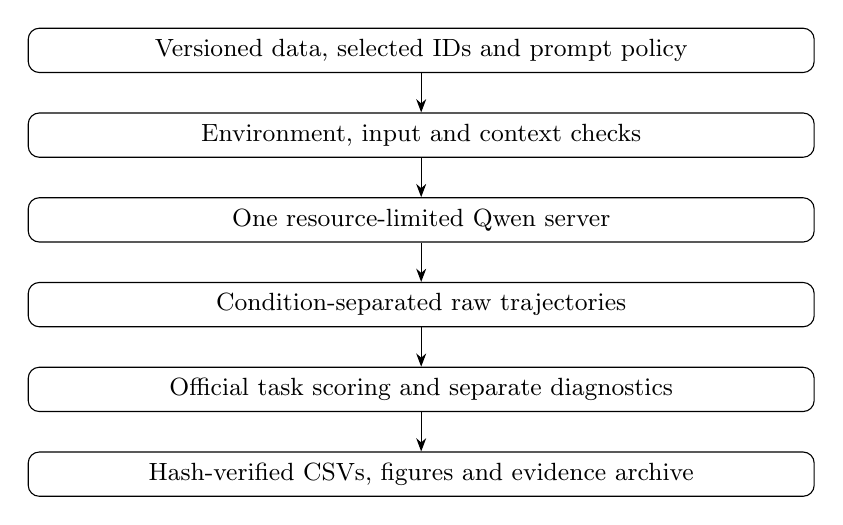
\begin{tikzpicture}[node distance=5mm, every node/.style={draw,rounded corners,align=center,font=\small,text width=.80\columnwidth,inner sep=4pt}, >={Stealth}]
\node (a) {Versioned data, selected IDs and prompt policy};
\node[below=of a] (b) {Environment, input and context checks};
\node[below=of b] (c) {One resource-limited Qwen server};
\node[below=of c] (d) {Condition-separated raw trajectories};
\node[below=of d] (e) {Official task scoring and separate diagnostics};
\node[below=of e] (f) {Hash-verified CSVs, figures and evidence archive};
\draw[->] (a)--(b);\draw[->] (b)--(c);\draw[->] (c)--(d);\draw[->] (d)--(e);\draw[->] (e)--(f);
\end{tikzpicture}
\caption{Implemented generation and analysis flow. Reference controls are offline software tests, not model predictions.}\label{fig:pipeline}
\end{figure}

Each run receives a fresh identifier. Status and file hashes are exported with logs, predictions and scores. On failure, diagnostic outputs are retained. Valid earlier trajectories are not overwritten to obtain favorable examples. This preservation is essential to distinguish software recovery from selective reporting of model performance.

\section{Computational Setup and Recovery}
\subsection{Observed environment}
Generation ran in user-operated Google Colab with a Tesla T4 exposing 15360 MiB GPU memory and approximately 12.67 GiB host RAM. We used a separate Python 3.12 virtual environment. The notebook kernel could remain on a different Python version; BFCL and vLLM were explicitly invoked through the virtual environment. Core versions are listed in Table~\ref{tab:environment}, and the complete observed package freeze is included with the repository.

\begin{table}[t]\caption{Observed core software and serving settings.}\label{tab:environment}\centering\small
\begin{tabular}{ll}\toprule
Component & Version or setting\\\midrule
Python & 3.12\\
torch / vLLM & 2.6.0 / 0.8.5\\
transformers / numpy & 4.51.3 / 1.26.4\\
tokenizers / huggingface\_hub & 0.21.4 / 0.36.2\\
qwen-agent / soundfile & 0.0.34 / 0.14.0\\
Precision / GPU fraction & FP16 / 0.85\\
Sequence and BFCL concurrency & One each\\
Recovery context cap & 24576 tokens\\
Chunked prefill & 2048 tokens\\
CPU swap / offload & 0 / 0 GiB\\\bottomrule
\end{tabular}
\end{table}

The model registry is \path{Qwen/Qwen3-4B-Instruct-2507-FC}; the underlying checkpoint omits \code{-FC}~\cite{qwencheckpoint}. The observed config revision was recorded. The development launch did not explicitly pin every remote artifact; we therefore avoid a stronger artifact-reproducibility claim. The prospective notebook pins the model, tokenizer and handler-side configuration to the recorded revision. Pinning records provenance but does not guarantee bitwise identical stochastic outputs across machines.

\subsection{Context-budget incident}
The initial comparative attempt used a 12288-token server cap. Vanilla completed, but a later general-review task required 8302 input tokens plus the preserved 4096-token answer allowance: 12398 tokens in total, exceeding the cap by 110. This was a serving-budget error, not a CUDA out-of-memory result or evidence of model accuracy. Checking only the first prompt had not prevented conversation history growth.

Recovery synchronized the handler's effective context with the server cap and added an explicit guard. The guard rejects a request when input tokens plus 4096 answer tokens and a two-token safety margin exceed the cap. It does not truncate history or silently reduce answer allowance. The cap was increased to 24576 under the same GPU memory fraction and single-sequence profile. A new output directory recorded recovery rather than overwriting the first attempt.

Eleven valid trajectories were reused and checked field-for-field against the source archive. Seven records were generated during recovery, including the failed inference retry and the checklist condition. This mixture is disclosed. The pilot is not a uniform-run experiment for timing, cache behavior or shared random-number stream analysis. The new prospective protocol avoids reusing these task records.

\subsection{Memory evidence and limits}
The successful recovery server profiler reported 7.61 GiB for model weights, 0.16 GiB activation peak and 4.57 GiB KV cache. These are profiler allocation quantities rather than continuous whole-system peak measurements. The largest observed prompt was 9161 input tokens; with the answer budget it remained below the recovered cap. The profile worked for these cases but does not guarantee fit for arbitrary BFCL histories or future model versions.

No CPU offload or swap was enabled, protecting the constrained host RAM budget. Model weights and server memory were not loaded into the notebook kernel merely to inspect logs. The same server served the three conditions sequentially. Fixed order and cache warm-up preclude a fair latency comparison, so no prompt speedup is claimed.

\section{Measured Development Results}
\subsection{Complete-task outcomes}
Table~\ref{tab:results} and Fig.~\ref{fig:tasks} report the official task outcomes. Every condition completed zero of six tasks. This supports the narrow observation that the added instructions did not yield full-task success on the inspected development set. It does not establish that schema guidance never helps, nor that the model performed every intermediate action incorrectly.

\begin{table}[t]\caption{Actual development complete-task outcomes.}\label{tab:results}\centering
\begin{tabular}{lrr}\toprule
Condition & Successes / tasks & Accuracy\\\midrule
Original & 0/6 & 0\%\\
General review & 0/6 & 0\%\\
Schema evidence & 0/6 & 0\%\\\bottomrule
\end{tabular}
\end{table}
\begin{figure}[t]\centering
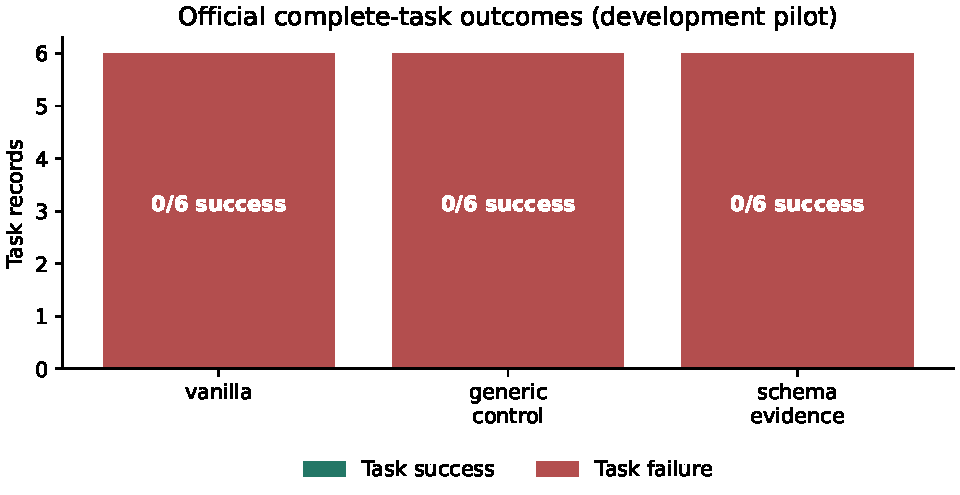
\includegraphics[width=\columnwidth]{figures/task_outcomes.pdf}
\caption{Observed task counts. The zero-success outcome is retained rather than replaced with favorable cases.}\label{fig:tasks}
\end{figure}

Across the 18 condition/task records, the first reported error types were 13 simulation-state mismatches, four execution-response mismatches and one force termination. These are first failures reported by the scorer, not exhaustive counts of every incorrect action in the conversations. Once a case fails at one point, later errors can be obscured by that first failure. Fig.~\ref{fig:failures} presents the counts without treating repeated variants as independent samples.

\begin{figure}[t]\centering
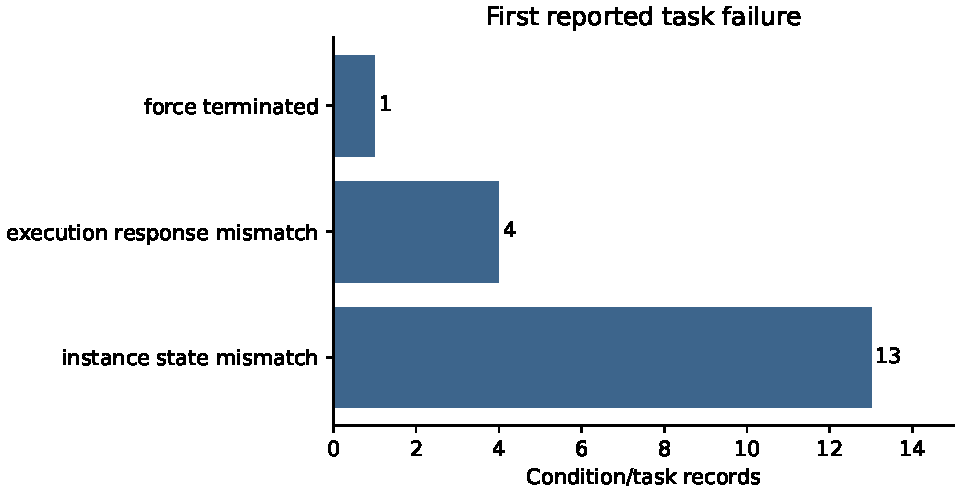
\includegraphics[width=\columnwidth]{figures/failure_types.pdf}
\caption{First reported failures across condition/task records. Counts do not identify a unique causal mechanism.}\label{fig:failures}
\end{figure}

\subsection{Concrete failure observations}
In vanilla base family 2, the model attempted to change into \code{document}, while the simulated directory was \code{documents}. The expected newly created file was absent from the evaluated state. This is a direct directory and task-completion failure, not evidence that a tool was unavailable. Other trajectories attempted copies from the wrong working directory or created an unexpected directory. Tool-call plausibility alone was insufficient to complete the workflow.

In the earlier smoke traces, copying a file was not equivalent to moving it. We also found that a function marked as excluded in metadata could still be visible in the actual model prompt. In the prompting path, a restored function was supplied in a later user message while the initial tool block remained unchanged. These observations motivate auditing model-visible history rather than deriving availability exclusively from one metadata field or the first tool block.

Similarly, an optional argument with a default value did not by itself establish that clarification was semantically necessary. Required-field checks and benchmark category names cannot substitute for verified intent labels. We therefore report the observable failures and preserve the distinction between operational no-call checks and a useful conversational explanation.

\subsection{Integrity and missingness}
All 203 files covered by the recovery manifest and all 62 covered by the nested source manifest matched their hashes. All 11 reused records matched their original content. The 18 final condition/task records had no recorded top-level inference exceptions. One general-review missing-parameter record was force-terminated after tool-loop behavior; it remains a task failure and is not silently removed as an infrastructure exception.

That force-terminated record lacks usable saved decoded evidence for a secondary no-call comparison. It is therefore explicitly unavailable for that measure. The complete-task denominator and the secondary decoded-evidence denominator are different for a documented reason. We do not turn missing evidence into successful abstention or compute an unqualified common accuracy across incompatible denominators.

\section{Metric Reproduction and Software Controls}
\subsection{Three distinct behavior definitions}
The official complete-task score, strict no-call compliance and published act/hold scoring target different properties. A strict no-call audit asks whether there are any decoded calls at a turn whose reference list is empty. In our development traces, all 11 intervention records with available decoded outputs contained calls at that turn. This yields 0/11 compliance, with the force-terminated record separately unavailable.

The released act/hold definition instead asks whether the model attempted a call labeled state-changing when the anchor was complete, and attempted no such call when the twin lacked information. Read-only navigation or inspection can be permitted under that definition. The labels and eligibility certification belong to the published work; we did not independently annotate all functions or prove useful clarification quality. Calls that fail during execution can still count as attempts.

Table~\ref{tab:decision} reports our post-hoc application of the original released scorer. Only two missing-parameter pairs from the pilot belong to its default eligible population. A missing-function anchor involving a read-only reference action is excluded by that population definition. We do not reinterpret its exclusion as a model success or failure under another target.

\begin{table}[t]\caption{Attributed published decision score on only two eligible development pairs per condition. Post-hoc; no significance claim.}\label{tab:decision}\centering\small
\begin{tabular}{lrrrr}\toprule
Condition & $n$ & Act & Hold & Mean\\\midrule
Original & 2 & 50\% & 50\% & 50\%\\
General review & 2 & 50\% & 0\% & 25\%\\
Schema evidence & 2 & 100\% & 50\% & 75\%\\\bottomrule
\end{tabular}
\end{table}

Both raw anchor turns were present for the selected pairs. Removing the missing twin's reference-empty turn restored its complete reference trajectory. Where official decoded outputs existed, the published parser's function-name sequence matched that saved sequence. The force-terminated general-review record had a raw anchor but lacked the official decoded sequence for this cross-check. Argument-level parser equivalence was not established. These checks and limitations accompany the result rather than being hidden behind one percentage.

The numerical checklist advantage in the secondary mean is not evidence of a reliable improvement. It arises on two inspected pairs, with the same prompt-length, order and provenance limitations as the rest of the pilot. The result is useful because it shows why a task-level floor does not fully describe lower-level behavior. It does not justify selecting a favorable metric after seeing the data and declaring a method successful.

\subsection{Reference controls}
We executed CPU-only synthetic reference controls using original BFCL checker and tool code. For the six development cases, author reference calls passed both a batched-per-turn and one-call-per-step layout. No reference execution exceptions were recorded. Six empty-action negative controls were rejected by execution checking, and four injected-call controls at no-call turns were rejected by the standalone irrelevance checker.

These tests supplied author answers deliberately. They do not show that Qwen achieved 6/6 accuracy. They establish specific software behavior on selected inputs. A separate exception check is important: an early synthetic identifier beginning with a digit produced invalid Python execution expressions even though reference-versus-reference equality could still pass. An alphabetic prefix corrected the control, and only the corrected run is reported as successful.

\subsection{Dispatch integration control}
Inspecting the pinned evaluation runner showed that it imports but does not invoke the standalone multi-turn irrelevance checker in its per-case evaluation function. The execution checker skips state/response comparison at empty-reference turns. Consequently, the existence of a standalone checker is not evidence that official full-task scoring enforces strict absence of calls there.

To test that integration boundary, we extracted the unchanged original evaluation function using Python AST and supplied an identity decoder for deliberate synthetic call lists. The real execution checker accepted six references. In all four intervention cases, inserting a read-only \code{pwd()} at an empty-reference turn also passed the evaluation function, while separately invoking the irrelevance checker rejected the addition. This is a controlled statement about the pinned implementation, not a full production decoder or CLI reproduction.

The earlier direct-checker tests remain valid, but their interpretation is narrower than a claim that every component was integrated into official scoring. Making this correction explicit is part of baseline validation. Neither source inspection alone nor a successful program exit would have established the distinction without checking which function the runner actually uses.

\section{Discussion and Threats to Validity}
\subsection{What the outputs support}
The primary question has a clear development answer: no condition completed any selected task. The added instructions were present in actual inputs, yet task-level success remained at the floor. The traces show state-navigation and operation-substitution failures alongside intervention-turn calls. A reasonable hypothesis is that generic verbal checks do not reliably control long-horizon execution in this small model. However, the current experiment does not isolate that mechanism from task difficulty, prompt formulation or recovery conditions.

\subsection{Internal and external validity}
Internal validity is limited by unequal prompt lengths, fixed condition order, shared-server randomness and mixed 12K/24K development provenance. The general-review condition is not a calibrated policy, and the checklist differs from vanilla in more than one explanatory element. Thus the pilot does not isolate the causal effect of schema evidence. The same task variants share underlying families; no independent-record statistical test is appropriate.

External validity is limited by one model and two comparative development families. We did not sample a representative full-benchmark population, repeat independent model seeds or establish behavior across domains and model scales. Benchmark contamination and alternative valid trajectories also remain possible. The synthetic reference tests show that the selected references execute; they do not prove every dataset item is uniquely specified or that all valid user-satisfying trajectories receive credit.

Measurement validity is limited by the distinctions above. Useful clarification prose is not scored. Strict no-call compliance can reject harmless exploration, while attempted state-changing behavior can count an unsuccessful call as acting. State/response checks can fail early, hiding later behavior. The published function labels and pair certification are inherited and attributed, not replaced with an unverified semantic oracle.

\subsection{Prospective extension and amendment policy}
ATR-P07-v1 fixes two new families, 89 and 73, before viewing their model outputs. Eligibility requires the published mutator-pair definition for both missing categories, exclusion of inspected families and previously unequal initial states, and deterministic hash sorting. Both selected families are vehicle-control tasks, which narrows rather than broadens domain claims. Their six author reference trajectories passed a CPU preflight. The protocol, selected input/reference hashes, notebook and budget were committed before generation.

The primary prospective comparison is checklist minus general review in official task success, accompanied by raw counts. The same three conditions and one fixed serving profile are preserved. The protocol allows negative outcomes and does not promise significance from a small sample. Any context or serving failure must be reported as incomplete execution, not silently replaced with an easier case. Changing prompts, IDs, metrics or limits after results requires a dated amendment and separation of prior observations.

At the time of this manuscript version, that new GPU evaluation is pending. No prospective table or anticipated numerical result is fabricated. The current paper is an evidence-based report of completed development work, with a transparent path to completing the separately frozen stage. A later revision may incorporate its genuine outputs without rewriting the historical pilot as a pre-frozen experiment.

\section{Reproducibility and Human--AI Accountability}
\subsection{Artifact structure and reruns}
The repository retains source pins, the observed dependency freeze, exact prompt scripts, notebooks, configurations, raw output archives, per-case scores, CSV analyses and paper sources. The analysis script verifies archive hashes, complete-run status, exact unique IDs, inference exceptions and score-header counts before writing figures. It was run on the authentic recovery archive. Commands that are prepared but not executed, including the exact cold dependency replay, are marked as requiring testing.

The latest notebook reuses the verified virtual environment on a warm Colab runtime and checks the core versions rather than upgrading packages automatically. A cold path is supplied for reconstruction with observed pins, but local syntax checks are not presented as a successful GPU installation. Server, tokenizer and handler configuration revisions are pinned for the prospective run. Source and data hashes detect silent differences. The notebook exports diagnostic output on failure and stops only its own server process group.

Reproducing a configuration does not mean producing byte-identical model text. Driver behavior, external artifact access, stochastic generation and shared server random streams remain relevant. The paper preserves enough provenance to inspect differences instead of promising impossible determinism. Model weights are not included in the submission package; their access and licensing remain governed by the original provider.

\subsection{AI assistance and student responsibility}
ChatGPT assisted with source inspection, notebook preparation, debugging, analysis and writing. The user executed the GPU notebooks and supplied genuine errors and archives. CPU controls and offline analyses ran in the assistant workspace. Exact historical chatbot model versions are not independently established for every turn and are not invented. The AI-use ledger distinguishes direct quotations from activity summaries and links decisions to actual code and evidence.

The development process exposed genuine limitations of AI assistance: a missing transitive import, an incomplete initial context preflight, an invalid synthetic identifier, an overly broad inference about checker integration and overly broad completion language before the original assignment was rechecked. These issues were corrected using tracebacks, actual source, executed controls and the instruction sheet. Their existence is not concealed by a polished narrative.

Student understanding cannot be certified by an assistant-generated report. A separate walkthrough identifies the model/data flow, context guard, scoring distinctions and representative failures to explain in a five-minute demonstration. The student must review that material and provide an authentic personal reflection. No fictional account of independent coding, annotation or human reasoning is substituted for that requirement.

\section{Conclusion}
This resource-constrained BFCL pilot produced no complete-task successes under original, general-review or schema-evidence prompting on six development tasks per condition. Failure analysis exposed ordinary state-tracking and execution problems alongside intervention-turn behavior. Reproducing a published act/hold metric and testing actual evaluator dispatch showed why task success, strict no-call compliance and attempted state changes must be interpreted separately. The small secondary percentages do not establish improvement. The artifacts preserve authentic failures, recovery provenance and executed controls, while a prospectively frozen evaluation remains explicitly pending. The result is a defensible implementation and measurement study with negative findings and reproducible evidence, rather than an unsupported novelty or performance claim.

\balance
\bibliographystyle{plain}
\bibliography{references}
\end{document}
